%%%%%%%%%%%%%%%%%%%%%%%%%%%%%%%%%%%%%%%%%
% NIH Grant Proposal for the Specific Aims and Research Plan Sections
% LaTeX Template
% Version 1.1 (26/12/19)
%
% This template originates from:
% http://www.LaTeXTemplates.com
%
% Original author:
% Erick Tatro (erickttr@gmail.com) with modifications by:
% Vel (vel@latextemplates.com)
%
% Adapted from:
% J. Hrabe (http://www.magalien.com/public/nih_grants_in_latex.html)
%
% License:
% CC BY-NC-SA 3.0 (http://creativecommons.org/licenses/by-nc-sa/3.0/)
%
%%%%%%%%%%%%%%%%%%%%%%%%%%%%%%%%%%%%%%%%%

%----------------------------------------------------------------------------------------
%	PACKAGES AND OTHER DOCUMENT CONFIGURATIONS
%----------------------------------------------------------------------------------------

\documentclass[11pt, notitlepage]{article} % Default font size and suppress title page

% \usepackage[utf8]{inputenc} % Required for inputting international characters
\usepackage[T1]{fontenc} % Output font encoding for international characters
% A note on fonts: As of 2019, NIH allows Arial, Georgia, Helvetica, and Palatino Linotype. Georgia and Arial are commercial fonts so you will need to use XeLaTeX and have them installed on your machine to use them. Palatino & Helvetica are available as free LaTeX packages so select the one you want and comment out the other.
\usepackage{palatino} % Palatino font
\linespread{1.05} % A little extra line spread is better for the Palatino font
% \usepackage{helvet} % Helvetica font
% \renewcommand*\familydefault{\sfdefault} % Use the sans serif version of the font

\usepackage{amsfonts, amsmath, amsthm, amssymb} % For math fonts, symbols and environments
\usepackage{graphicx} % Required for including images
\usepackage{booktabs} % Nice rules in tables
\usepackage{wrapfig} % Required for text to wrap around figures and tables
\usepackage[labelfont=bf]{caption} % Make figure numbering in captions bold
\usepackage[top=0.5in,bottom=0.5in,left=0.5in,right=0.5in]{geometry} % Page margins
\usepackage[style=numeric, sorting=nyt, sortcites=true]{biblatex}
\usepackage{color, colortbl, soul}
\usepackage{tabularx}
\usepackage{array}
\usepackage{caption}
\usepackage[colorlinks=false]{hyperref}

\newcommand{\myfloatalign}{\centering} % to be used with each float for alignment

\definecolor{Gray}{gray}{0.9}
\addbibresource[]{mybib.bib}
\pagestyle{empty} % Suppress headers and footers

\hyphenation{ionto-pho-re-tic iso-tro-pic fortran} % Specifies custom hyphenation points for words or words that shouldn't be hyphenated at all
\def\eg{{\emph{e.g.,}}~}
\def\ie{{\emph{i.e.,}}~}
\def\cf{{\emph{cf.,}}~}

%---------------------------------------------------------------------

\begin{document}

%----------------------------------------------------------------------------------------
%	SPECIFIC AIMS
%----------------------------------------------------------------------------------------

\section*{Specific Aims}

The \textbf{objective} of this proposal is to directly and more completely characterize the perceptual experience of tinnitus using the novel application of a primary method for uncovering latent perceptual representations: reverse correlation.
Tinnitus is the perception of ringing, buzzing, or hissing in the ears, which can range from mild and transient to debilitating.
In the U.S. alone, it affects 45 million people per year, 30\% of which report their tinnitus to be moderate to severe.
A primary form of treatment habituation therapy that retrains a patient’s nervous system by habituating it to external sounds that mimic the perceptual experience of the tinnitus sound.
Habituation therapies require accurate estimates of patients’ tinnitus experience in order to promote patient outcomes.
There is a pressing need for new approaches to uncovering individuals’ perceptual experience of tinnitus,
because current estimation methods rely on strongly reductionist assumptions concerning the nature of tinnitus sounds, 
and produce results that are correspondingly biased and incomplete.
Reverse correlation holds promise in this regard,
as a primary method used to characterize neural tuning that is known to allow for unconstrained and unbiased estimation of latent neural representations
(\eg neural receptive fields) \cite{ringachReverseCorrelationNeurophysiology2004, nishimotoReceptiveFieldProperties2006},
as well as higher-level cognitive representations, including psychophysical kernels that drive the top-down processes of perception 
(\eg face or phoneme recognition) \cite{gosselinSuperstitiousPerceptionsReveal2003,smithMeasuringInternalRepresentations2012,neriReceptivePerceptiveFields2006,ahumadaStimulusFeaturesSignal1971},
and even abstract psychological categories (\eg “male” vs. “female” faces)
\cite{brinkmanVisualisingMentalRepresentations2017,manginiMakingIneffableExplicit2004,ponsotCrackingSocialCode2018},
all on the basis of fairly simple stimulus-response data \cite{ljungMeasureLackFit1978,marmarelisWhiteNoiseMethodSystem1978}.
Despite its wide acceptance in other areas of inquiry, reverse correlation has not been brought to bear with respect to uncovering tinnitus experience.

Our \textbf{long-term goal} is to directly uncover and more completely characterize the perceptual experience of tinnitus using the demonstrated capabilities of the reverse correlation approach.
Our guiding hypothesis is that reverse correlation will produce estimates of tinnitus percepts that are substantially more rich, individualized and unbiased than currently possible using existing approaches. The rationale is that high quality characterization of tinnitus percepts can promote detailed assessment of tinnitus, helping to explain individual variability in tinnitus experience, and ultimately informing individualized treatment through enhanced habituation therapies. The proposed work will simultaneously improve the efficiency of the reverse correlation method itself, further enhancing its potential for adoption in clinical settings. We will test our central hypothesis and attain our objective via the following specific aims:

\begin{description}
	\item[Aim \#1: Uncover and reconstruct cognitive representations of tinnitus]{} 
\end{description}

To reconstruct perceptual representations of tinnitus using a novel reverse correlation procedure. Participants with tinnitus will be presented with richly varying stimuli in the context of a yes-no behavioral response paradigm. Perceptual representations can be estimated by regressing observed responses against the stimuli over many trials. Reconstructed representations will be compared to conventional estimates of tinnitus from the same participants. Expected outcome: reconstructed representations of tinnitus will more detailed and less biased than any those obtained through conventional methods.

\begin{description}
	\item[Aim \#2: Develop efficient reconstruction algorithm for cognitive representations using compressive sensing]{} 
\end{description}

To enhance the efficiency of the reverse correlation procedure using compressive sensing, which substantially reduces the number of trials required to accurately reconstruct perceptual representations. We will use compressive sensing to more efficiently and more accurately reconstruct cognitive representations using data obtained in Aim \#1. Expected outcome: compressive sensing is expected to improve efficiency of the reverse correlation procedure by up to 90\%.
% The reverse correlation and compressive sensing framework will be released
% as an open-source software implementation for use by the research community.
% Our pilot data demonstrates that compressive sensing affords a 90\% decrease
% in the number of trials for equivalent resultant latent representation.


\begin{description}
	\item[Aim \#3: Characterize and interpret cognitive representations of tinnitus]{} 
\end{description}

To characterize variability in perceptual representations of tinnitus between participants and over time. We will use unsupervised machine learning techniques to reveal latent similarities between tinnitus representations, and subsequently cluster those into distinct categories. Expected outcome: Unsupervised machine learning will identify distinct categories of tinnitus, which will allow us to further improve the effiency and accuracy of uncovering tinnitus representations through improved stimulus generation and representation classification. 


% Dimensionality reduction algorithms will reveal latent similarities between
% tinnitus representations which will be subtyped using a data-driven approach.

% Our compressive sensing framework will allow for rapid data acquisition from participants.
% We will characterize cognitive representations of tinnitus between participants and over time.
% What is the space of tinnitus cognitive representations?
% Are there subtypes or clusters on a lower dimensional manifold?
% We will employ dimensionality reduction and clustering algorithms to represent and visualize the data,
% providing direct insight into commonalities and variability of tinnitus experience in and between subjects.

%----------------------------------------------------------------------------------------
%	SIGNIFICANCE
%----------------------------------------------------------------------------------------

\newpage

\section*{A. Significance}

Tinnitus, the perception of ringing, buzzing, or hissing in the ears when no external sound is present,
is a health condition estimated to affect 10-15\% of adults worldwide \cite{henryTinnitusEpidemiologicPerspective2020}.
The condition is highly heterogeneous and can range from mild and transient to debilitating and constant.
In the U.S., tinnitus affects approximately one in ten Americans, with 7.2\% of those rating their tinnitus as severe (\cite{bhattPrevalenceSeverityExposures2016}.
Tinnitus can be perceived unilaterally or bilaterally and may differ over time, even within individuals.
This heterogeneity in characterization has important implications for research
and clinical practice.
Identifying patterns in how tinnitus sounds and its relationship to hearing may aid in identifying
different forms of tinnitus and revealing their underlying mechanisms.
However, the subjective nature of characterizing tinnitus makes it difficult
to reliably define and measure \cite{vajsakovicPrinciplesMethodsPsychoacoustic2021}.

Current methods to determine cognitive representations of tinnitus
are inefficient and introduce bias, resulting in a lack of standardization in tinnitus assessment \cite{henryTinnitusEpidemiologicPerspective2020}.
One common method is the alternate forced-choice (AFC) paradigm task, which asks the patient to determine which of two sounds
is closer to their tinnitus percept
\cite{henryComparisonTwoComputerautomated2001,henryComputerautomatedTinnitusAssessment2004,henryComputerautomatedTinnitusAssessment2013,korthOneStepCloser2020}.
Recent computer and methodological advances have made the test more portable and efficient,
but the AFC paradigm still relies on assumptions about the subject's tinnitus percept.
Tinnitus percepts are too heterogeneous to be represented by pure tones or small-envelope waveforms.
\autoref{fig:tinnitusexamples} displays spectrograms of example tinnitus percepts
from the American Tinnitus Association website,
showing the heterogeneity of tinnius percepts as well as their richness in frequency spectra and temporal characteristics.
Adequately sampling the psychoacoustic space of possible tinnitus percepts via an AFC task is unfeasible.
Other approaches have attempted to capture the richness of tinnitus percepts using likeness measures,
in which the subject rates whether a presented stimulus is part of their tinnitus percept or not \cite{norenaPsychoacousticCharacterizationTinnitus2002}.
While these methods capture more features of cognitive representations of tinnitus,
they are time-consuming and limited by the aural skills of the subject \cite{vajsakovicPrinciplesMethodsPsychoacoustic2021}.
Both AFC and likeness measures involve the subject comparing an external stimulus to their cognitive representation of the tinnitus percept,
however AFC tasks introduce biases by artificially limiting the stimulus space and likeness measures are time-consuming.
\emph{We believe that a novel reverse correlation-based approach will produce efficient and unbiased cognitive representations of tinnitus percepts}
\cite{gosselinSuperstitiousPerceptionsReveal2003}.

\begin{figure}[h] % Figure at bottom of the page ([b] argument, could be "t" for top or "h" for here)
	\centering
	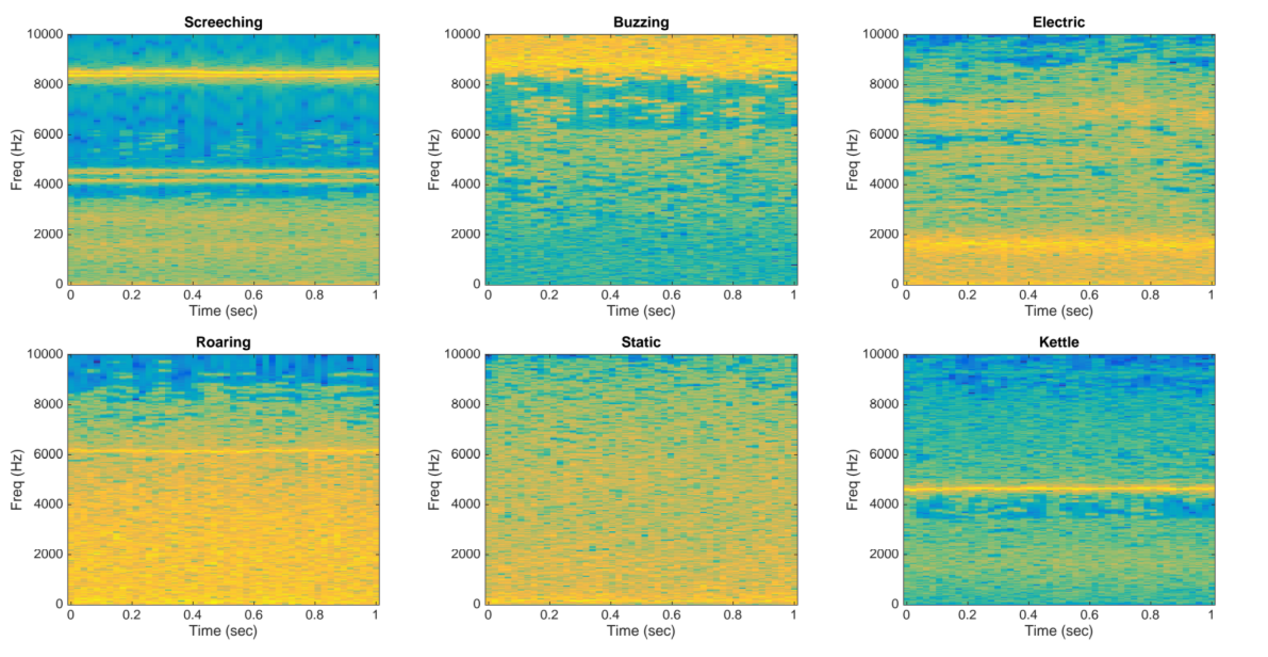
\includegraphics[width=0.8\textwidth]{Figures/Figures_tinnitus_6.png}
	\caption{Examples of tinnitus spectrograms from the American Tinnitus Association website \cite{Symptoms2015}.
	These spectrograms are heterogeneous as well as high-dimensional; the signals contain many frequency bands and vary over time.}
	\label{fig:tinnitusexamples}
\end{figure}

Reverse correlation allows for unconstrained and unbiased
characterization of latent representations directly from stimulus-response data by eliciting responses to
richly varying stimuli, such as white noise \cite{marmarelisWhiteNoiseMethodSystem1978, nishimotoReceptiveFieldProperties2006}.
Rich stimuli, by virtue of the fact that they are inherently vague, force the top-down process to exert a clearly
measurable influence on responses. Latent representations that drive the top-down process can then be
estimated by regressing observed responses against the stimuli over many trials \cite{mineaultImprovedClassificationImages2009}.
Reverse correlation, as a method, is powerful enough to characterize any aspect of neurological,
cognitive or psychological function that can be modeled as a transductive process \cite{ringachReverseCorrelationNeurophysiology2004}.
It has become a primary method used to characterize the latent representations encapsulated in neural tuning
(\eg receptive fields; \cite{ringachReverseCorrelationNeurophysiology2004}), and is closely related to the widely-used ``white noise approach'' to
characterizing physiological \cite{marmarelisWhiteNoiseMethodSystem1978} and engineering \cite{ljungMeasureLackFit1978} systems. 

Reverse correlation has been increasingly used for inferring higher-level cognitive representations as well,
including psychophysical kernels that drive the top-down processes of perception
\cite{ahumadaStimulusFeaturesSignal1971, neriReceptivePerceptiveFields2006,gosselinSuperstitiousPerceptionsReveal2003,smithMeasuringInternalRepresentations2012}, 
and even abstract psychological
categories (\eg ``male'' vs. ``female'' faces; \cite{brinkmanVisualisingMentalRepresentations2017,manginiMakingIneffableExplicit2004,ponsotCrackingSocialCode2018}.
Recent work in vision has demonstrated that
reverse correlation can effectively characterize cognitive representations underlying letter and face
recognition \cite{gosselinSuperstitiousPerceptionsReveal2003,liuSeeingJesusToast2014}.
One speech study has also estimated steady-state representations of vowels /a/
and /i/ using a closely-related paradigm to the one proposed here (Fig 2B; \cite{brimijoinInternalRepresentationVowel2013}). Our
proposed use of reverse correlation in the domain of speech expands on classic efforts to understand
top-down processing in speech with the presentation of rich, vague stimuli to elicit responses from
listeners \cite{warrenAuditoryIllusionsConfusions1970,vokeySubliminalMessagesDevil1985}.
These studies provide clear evidence that rich
stimuli, such as white noise, are sufficient to engage the top-down process, even if they do not attempt to
characterize the latent representations.

Incomplete characterizations of cognitive representations impoverish our scientific understanding of tinnitus,
weaken causal explanations for its etiology, and hinder progress towards effective treatments.
Reverse correlation shows promise to provide a more complete characterization of cognitive representations of tinnitus
and is applicable to other psychophysical domains as well.
Directly characterizing complex representations of tinnitus can enable more effective, targeted treatments,
reveal insights about subtypes of the condition, and pave the way for new tinnitus-masking assistive devices.
Fully characterizing a high-dimensional representation of tinnitus will improve causal explanations
for currently unexplained variability in tinnitus experience both between subjects and within single subjects over time.

% \begin{description}
% 	\item[A.3. Rigor of the Prior Research]{}
% \end{description}

\emph{The premise of the proposed work is that reverse correlation will deliver unbiased estimates
of cognitive representations of tinnitus. Furthermore, that compressive sensing will dramatically
increase the efficiency of experiments, resulting in convergent cognitive representations
in a fraction of the samples.}

The evidence for this premise is first based on well-established studies using reverse correlation
to derive cognitive representations of sounds and symbols.
Reverse correlation has been applied to infer cognitive representations from letters
\cite{gosselinSuperstitiousPerceptionsReveal2003}, vowel sounds \cite{brimijoinInternalRepresentationVowel2013},
and faces \cite{brinkmanVisualisingMentalRepresentations2017,smithMeasuringInternalRepresentations2012}.
More broadly, it has been applied to infer the shape of receptive fields
in linear transducers and spiking neurons \cite{ringachReverseCorrelationNeurophysiology2004}.
The reverse correlation paradigm makes minimal assumptions about the derived cognitive representation
since the subject is presented with high-dimensional random input.
A large number of stimulus-response samples are typically required for accurate
reconstruction of cognitive representations using conventional techniques. To address this inefficiency,
studies often limit the richness of stimuli, or impose strict constraints on the reconstructions, leading to
estimates that are biased or incomplete. However, recent advances in signal processing, most notably
a techniques known as compressive sensing, are leading to dramatic improvements the efficiency of
traditional sampling.

We propose to develop an advanced signal processing pipeline that will enable us to overcome
the inefficiencies of existing reverse correlation methods through the use of compressive sensing, a
recent advance in signal processing which has led to dramatic improvements the efficiency of traditional
sampling and signal estimation methods \cite{baraniukCompressiveSensingLecture2007}. Compressive sensing has recently gained
wide recognition in domains such as medical imaging \cite{graffCompressiveSensingMedical2015,lustigCompressedSensingMRI2008}, where
considerations of efficiency and bias reduction are critical. Compressive sensing holds promise to
similarly improve the efficiency of reverse correlation, without the drawback of biasing estimates. By
dramatically decreasing the number of trials needed for signal reconstruction, this technique will extend
the range of perceptual mechanisms that can be estimated. Moreover, compressive sensing can be
directly substituted for conventional, regression-based estimation, with no other required changes to
existing experimental protocols. Our ultimate objective is to develop and validate a compressive sensing
data processing pipeline - culminating in an open-source software tool – that will allow for efficient and
accurate reconstruction of latent representations using data obtained via the reverse correlation method.


% \begin{wraptable}{l}{5.5cm} % Example table with text wrapping around it
% 	\caption{Example Table}
% 	\begin{center}
% 		\begin{tabular}{l l r}
% 			\toprule
% 			\multicolumn{1}{c}{City} & {N\textsuperscript{a}} & {\%Silly}\\
% 			\midrule
% 			San Diego & 289 & 41\%\\
% 			Seattle & 262 & 32\%\\
% 			Galveston & 261 & 15\%\\
% 			St Louis & 269 & 7\%\\
% 			New York & 271 & 4\%\\
% 			Baltimore & 231 & 2\%\\
% 			\emph{Total} & 1,586 & 21\%\\
% 			\hline 
% 		\end{tabular}\\
% 		\footnotesize\textsuperscript{a}{All participants clowns.}
% 	\end{center}
% 	\label{tab:example}
% \end{wraptable}

% Referencing a table using its label: Table \ref{tab:example}. Maecenas consectetur metus at tellus finibus condimentum. Proin arcu lectus, ultrices non tincidunt et, tincidunt ut quam. Integer luctus posuere est, non maximus ante dignissim quis. Nunc a cursus erat. Curabitur suscipit nibh in tincidunt sagittis. Nam malesuada vestibulum quam id gravida. Proin ut dapibus velit. Vestibulum eget quam quis ipsum semper convallis. Duis consectetur nibh ac diam dignissim, id condimentum enim dictum. Nam aliquet ligula eu magna pellentesque, nec sagittis leo lobortis. Aenean tincidunt dignissim egestas. Morbi efficitur risus ante, id tincidunt odio pulvinar vitae. Proin ut dapibus velit. Vestibulum eget quam quis ipsum semper convallis. Duis consectetur nibh ac diam dignissim, id condimentum enim dictum.

% Curabitur tempus hendrerit nulla. Donec faucibus lobortis nibh pharetra sagittis. Sed magna sem, posuere eget sem vitae, finibus consequat libero. Cras aliquet sagittis erat ut semper. Aenean vel enim ipsum. Fusce ut felis at eros sagittis bibendum mollis lobortis libero. Donec laoreet nisl vel risus lacinia elementum non nec lacus. Nullam luctus, nulla volutpat ultricies ultrices, quam massa placerat augue, ut fringilla urna lectus nec nibh. Vestibulum efficitur condimentum orci a semper. Pellentesque ut metus pretium lacus maximus semper. Sed tellus augue, consectetur rhoncus eleifend vel, imperdiet nec turpis. Nulla ligula ante, malesuada quis orci a, ultricies blandit elit.

% In malesuada ullamcorper urna, sed dapibus diam sollicitudin non. Donec elit odio, accumsan ac nisl a, tempor imperdiet eros. Donec porta tortor eu risus consequat, a pharetra tortor tristique. Morbi sit amet laoreet erat. Morbi et luctus diam, quis porta ipsum. Quisque libero dolor, suscipit id facilisis eget, sodales volutpat dolor. Nullam vulputate interdum aliquam. Mauris id convallis erat, ut vehicula neque. Sed auctor nibh et elit fringilla, nec ultricies dui sollicitudin.

% \begin{wrapfigure}{r}{8.5cm} % Example figure with text wrapping around it
% 	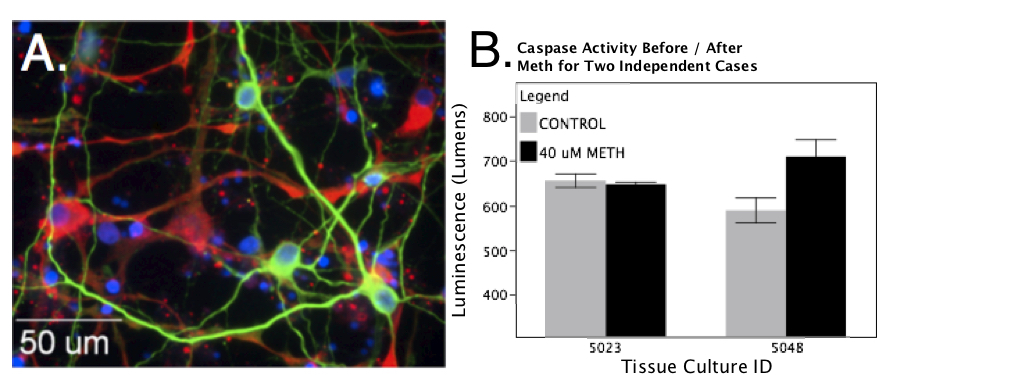
\includegraphics[width=8.2cm]{Figures/Fig1.jpg}
% 	\caption{\footnotesize Example wrapped figure. (A) Impressive microscopy image. (B) Impressive data.}
% 	\label{fig:example}
% \end{wrapfigure}

% Referencing a figure using its label: Figure \ref{fig:example}. Proin lobortis efficitur dictum. Pellentesque vitae pharetra eros, quis dignissim magna. Sed tellus leo, semper non vestibulum vel, tincidunt eu mi. Aenean pretium ut velit sed facilisis. Ut placerat urna facilisis dolor suscipit vehicula. Ut ut auctor nunc. Nulla non massa eros. Proin rhoncus arcu odio, eu lobortis metus sollicitudin eu. Duis maximus ex dui, id bibendum diam dignissim id. Aliquam quis lorem lorem. Phasellus sagittis aliquet dolor, vulputate cursus dolor convallis vel. Suspendisse eu tellus feugiat, bibendum lectus quis, fermentum nunc. Nunc euismod condimentum magna nec bibendum. Curabitur elementum nibh eu sem cursus, eu aliquam leo rutrum. Sed bibendum augue sit amet pharetra ullamcorper. Aenean congue sit amet tortor vitae feugiat. Vestibulum vestibulum luctus metus venenatis facilisis. Suspendisse iaculis augue at vehicula ornare. Sed vel eros ut velit fermentum porttitor sed sed massa. Fusce venenatis, metus a rutrum sagittis, enim ex maximus velit, id semper nisi velit eu purus.

% \begin{description}
% 	\item[A.3. Another subheading:]{optional subtitle.}
% \end{description}

% In congue risus leo, in gravida enim viverra id. Donec eros mauris, bibendum vel dui at, tempor commodo augue. In vel lobortis lacus. Nam ornare ullamcorper mauris vel molestie. Maecenas vehicula ornare turpis, vitae fringilla orci consectetur vel. Nam pulvinar justo nec neque egestas tristique. Donec ac dolor at libero congue varius sed vitae lectus. Donec et tristique nulla, sit amet scelerisque orci. Maecenas a vestibulum lectus, vitae gravida nulla. Proin eget volutpat orci. Morbi eu aliquet turpis. Vivamus molestie urna quis tempor tristique. Proin hendrerit sem nec tempor sollicitudin.

% \begin{figure}[b] % Figure at bottom of the page ([b] argument, could be "t" for top or "h" for here)
% 	\centering
% 	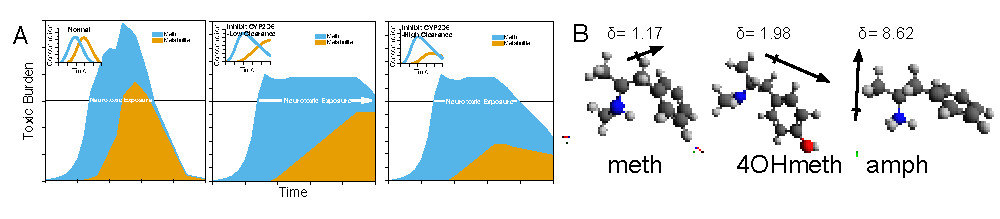
\includegraphics[scale = .80]{Figures/Fig2.pdf}
% 	\caption{\footnotesize Big Figure legend Big Figure legend Big Figure legend Big Figure legend Big Figure legend Big Figure legend Big Figure legend Big Figure legend Big Figure legend.}
% 	\label{fig2}
% \end{figure}

% Fusce eleifend porttitor arcu, id accumsan elit pharetra eget. Mauris luctus velit sit amet est sodales rhoncus. Donec cursus suscipit justo, sed tristique ipsum fermentum nec. Ut tortor ex, ullamcorper varius congue in, efficitur a tellus. Vivamus ut rutrum nisi. Phasellus sit amet enim efficitur, aliquam nulla id, lacinia mauris. Quisque viverra libero ac magna maximus efficitur. Interdum et malesuada fames ac ante ipsum primis in faucibus. Vestibulum mollis eros in tellus fermentum, vitae tristique justo finibus. Sed quis vehicula nibh. Etiam nulla justo, pellentesque id sapien at, semper aliquam arcu. Integer at commodo arcu. Quisque dapibus ut lacus eget vulputate.

% Vestibulum sodales orci a nisi interdum tristique. In dictum vehicula dui, eget bibendum purus elementum eu. Pellentesque lobortis mattis mauris, non feugiat dolor vulputate a. Cras porttitor dapibus lacus at pulvinar. Praesent eu nunc et libero porttitor malesuada tempus quis massa. Aenean cursus ipsum a velit ultricies sagittis. Sed non leo ullamcorper, suscipit massa ut, pulvinar erat. Aliquam erat volutpat. Nulla non lacus vitae mi placerat tincidunt et ac diam. Aliquam tincidunt augue sem, ut vestibulum est volutpat eget. Suspendisse potenti. Integer condimentum, risus nec maximus elementum, lacus purus porta arcu, at ultrices diam nisl eget urna. Curabitur sollicitudin diam quis sollicitudin varius. Ut porta erat ornare laoreet euismod. In tincidunt purus dui, nec egestas dui convallis non. In vestibulum ipsum in dictum scelerisque.

% \begin{description}
% 	\item[A.4. Yet another subheading.]{}
% \end{description}

% Aenean feugiat pellentesque venenatis. Sed faucibus tristique tortor vel ultrices. Donec consequat tellus sapien. Nam bibendum urna mauris, eget sagittis justo gravida vel. Mauris nisi lacus, malesuada sit amet neque ut, venenatis tempor orci. Curabitur feugiat sagittis molestie. Duis euismod arcu vitae quam scelerisque facilisis. Praesent volutpat eleifend tortor, in malesuada dui egestas id. Donec finibus ac risus sed pellentesque. Donec malesuada non magna nec feugiat. Mauris eget nibh nec orci congue porttitor vitae eu erat. Sed commodo ipsum ipsum, in elementum neque gravida euismod. Cras mi lacus, pulvinar ut sapien ut, rutrum sagittis dui. Donec non est a metus varius finibus. Pellentesque rutrum pellentesque ligula, vitae accumsan nulla hendrerit ut.

% In mi mauris, finibus non faucibus non, imperdiet nec leo. In erat arcu, tincidunt nec aliquam et, volutpat eget nisl. Vivamus id eros scelerisque est condimentum condimentum at at ligula. Proin blandit sapien ac bibendum faucibus. Nunc sem elit, blandit in lectus vitae, lacinia hendrerit risus. Donec efficitur elementum massa, eget interdum nunc porttitor sed. Aenean porttitor gravida nibh, vel bibendum tellus. Nunc fermentum lobortis nunc. Cras aliquet odio mauris, eget lobortis metus lacinia sit amet. Maecenas id elit eu orci ornare ultricies. Sed consequat turpis id accumsan malesuada. Fusce varius imperdiet ex, vel sodales purus scelerisque id. Morbi ut tellus interdum, laoreet leo non, dignissim odio. Nunc vel quam diam. Sed eu tortor in dolor mattis rhoncus.

%----------------------------------------------------------------------------------------
%	INNOVATION
%----------------------------------------------------------------------------------------

\section*{B. Innovation}

The proposed project is innovative for several reasons.
First, we will leverage interdisciplinary collaboration between engineering (Adam Lammert)
and hearing science (Ben Parrell) to characterize tinnitus to inform clinical care.
Second, we will apply reverse correlation to the tinnitus domain in a novel application,
which promises to deliver unbiased, high-dimensional estimates of cognitive representations of tinnitus.
Third, we will develop a signal processing pipeline to leverage compressive sensing
to acquire accurate estimates of cognitive representations of tinnitus using significantly fewer samples.
This pipeline will save experimenters and subjects time and will enable researchers
to collect data from more subjects and from individual subjects over time.
We will release our open-source software tool online with bindings to popular scientific computing languages.

%----------------------------------------------------------------------------------------
%	APPROACH
%----------------------------------------------------------------------------------------

\section*{C. Approach}

In the proposed project, we will use reverse correlation to reveal unbiased high-dimensional
representations of tinnitus and further characterize the condition
using dimensionality-reduction and density-based clustering.
We will use data regarding the space of tinnitus Representations
to iteratively improve our stimulus generation and representation classification algorithms.
In \emph{Aim \#1}, we will develop and run an experimental paradigm
in which tinnitus patients listen to noisy stimuli and perform an alternate forced-choice task
answering the question, ``Does this sound like your tinnitus?''
Instead of using limited, preconstructed stimuli, we will randomly sample from a distribution.
Reverse correlation frees us from the methodological constraint of imposing strong \emph{a priori}
assumptions about the tinnitus percept.
In \emph{Aim \#2}, we will develop an open-source signal processing pipeline
to reconstruct cognitive representations of tinnitus using compressive sensing.
Compressive sensing holds promise to dramatically reduce the number of samples
needed for accurate reconstruction, enabling us to run more experimental subjects for Aim \#1,
and retest subjects to examine the stability of cognitive representations of tinnitus over time.
\emph{Aim \#3} contextualizes reconstructed cognitive representations of tinnitus
by visualizing underlying subtypes or clusters on a lower dimensional manifold.
We will employ dimensionality reduction and clustering algorithms to represent and visualize the data,
providing direct insight into commonalities and variability of tinnitus experience in and between subjects.
Furthermore, we will use information about the distribution of representations
to iteratively improve our stimulus generation and data-driven subtype classification processes.

% \begin{description}
% 	\item[C.1. Aim \#1]{Uncover and reconstruct cognitive representations of tinnitus} 
% \end{description}

\subsection*{C. Aim \#1: Uncover and reconstruct cognitive representations of tinnitus}

In this aim, we will identify high-dimensional cognitive representations of tinnitus using reverse correlation.
Current methods for estimating cognitive representations of tinnitus fall broadly into three primary categories,
each of which has limitations (\autoref{tab:approaches}).

Two common approaches are alternate forced choice tasks with constructed stimuli
and likeness measures.
In the former experimental paradigm,
the experimenter presents participants with multiple samples of auditory stimuli that vary in well-characterized
and often highly-constrained ways, along specific dimensions (\eg pure tone frequency, width of spectral envelope)
that are known to be, or are hypothesized to be, relevant to tinnitus representation or masking
\cite{vajsakovicPrinciplesMethodsPsychoacoustic2021,henryMeasurementTinnitus2016}.
The subject then makes a choice between stimuli.
While new methodological advances in experiment design and technology have streamlined this approach
\cite{korthOneStepCloser2020,henryComputerautomatedTinnitusAssessment2004,henryComputerautomatedTinnitusAssessment2013},
it is still constrained by \emph{a priori} assumptions about the nature of tinnitus percepts.
In contrast, likeness approaches use subjective judgment tasks,
in which the subject rates how much (if at all) a presented stimulus is part of or masks their tinnitus percept
\cite{norenaPsychoacousticCharacterizationTinnitus2002}.
While likeness measures provide more complete reconstructions of tinnitus cognitive representations,
likeness tests are time-consuming and generally not used in clinical practice
\cite{vajsakovicPrinciplesMethodsPsychoacoustic2021}.

A third, more recent approach to uncovering cognitive representations is to employ neuroimaging
(\eg fMRI) to identify neural activation patterns indicative of tinnitus.
In investigations of functional connectivity in tinnitus patients,
resting-state fMRI measures were found to be replicable and reliable,
though no explicit representations have been proposed
\cite{husainReplicabilityNeuralBehavioral2019}.
This approach is also
limited, in that it can only uncover representations that have a definite, localized seat in the brain.
Cognitive representations, by contrast, are commonly understood to be constructs that need not have
such a localized neural seat by definition, and which can best be revealed through analyzing behavior.

The highly-constrained nature of stimuli used in the forced selection approach necessarily results
in recovered representations that are correspondingly constrained and typically low-dimensional. It has
long been known, however, that representations limited to only a few dimensions are insufficient to
account for the full richness of tinnitus experiences
\cite{vajsakovicPrinciplesMethodsPsychoacoustic2021,henryMeasurementTinnitus2016}.
Subjective judgment experiments yield more informative reconstructions but are time-consuming to employ.
The nature of subjective judgment
approach is such that it is best suited to uncover relations between perceptual categories, rather than
characterizing cognitive representations directly, and thus provides limited information about how
perceptual similarity comes about. While some of the recovered dimensions along which stimuli differ in
these tasks correlate with frequently assumed dimensions of representation (\eg frequency and pitch to mask tinnitus percept),
some recovered dimensions of contrast have no known characterization.
Moreover, this approach is fundamentally limited by the precise stimuli presented to participants, and
therefore may not systematically explore the entire space of perceptually-meaningful variables.

% \begin{table}[h]
% 	\centering
% 	\begin{tabular}{| >{\raggedright}p{35mm} >{\raggedright\arraybackslash}p{40mm} >{\raggedright\arraybackslash}p{45mm} >{\raggedright\arraybackslash}p{50mm}|} 
% 		\hline
% 		Approach & Stimulus & Measurements & Output \\ [0.5ex] 
% 		\hline
% 		\rowcolor{Gray} Forced selection & Constructed stimuli, constrained variation & Subjective choice & Representation with \newline defined acoustic properties \\
% 		Likeness measures & Constructed stimuli, constrained variation & Subjective ratings & Frequency spectra \\
% 		\rowcolor{Gray} Neural monitoring & N/A & Neural signals (\eg fMRI) & Correlation maps in localized brain regions, functional connectivity maps \\
% 		\textbf{Reverse Correlation} & Constructed stimuli, unconstrained variation & Response classification (\eg present/absent) & Representations best explaining classification behavior \\
% 		\hline
% 	\end{tabular}
% 	\caption{Comparison of approaches for estimating cognitive representations.
% 	Each approach has benefits and limitations regarding stimuli, measurements, and output.
% 	The proposed approach, featured in the final row, is the only approach that can directly
% 	uncover a time-frequency map of the cognitive representation that best explains tinnitus percepts.}
% 	\label{table:1}
% \end{table}

\begin{table}[h]
	\myfloatalign
	\begin{tabularx}{\textwidth}{>{\raggedright}p{35mm} >{\raggedright\arraybackslash}p{40mm} >{\raggedright\arraybackslash}p{45mm} >{\raggedright\arraybackslash}p{50mm}}
		\toprule
		\textbf{Approach} & \textbf{Stimulus} & \textbf{Measurements} & \textbf{Output} \\ [0.5ex] 
		\rowcolor{Gray} Forced selection & Constructed stimuli, constrained variation & Subjective choice & Representation with \newline defined acoustic properties \\
		Likeness measures & Constructed stimuli, constrained variation & Subjective ratings & Frequency spectra \\
		\rowcolor{Gray} Neural monitoring & N/A & Neural signals (\eg fMRI) & Correlation maps in localized brain regions, functional connectivity maps \\
		\textbf{Reverse Correlation} & Constructed stimuli, unconstrained variation & Response classification (\eg present/absent) & Representations best explaining classification behavior \\
		\bottomrule
	\end{tabularx}
	\caption[Approaches]{Comparison of approaches for estimating cognitive representations.
	Each approach has benefits and limitations regarding stimuli, measurements, and output.
	The proposed approach, featured in the final row, is the only approach that can directly
	uncover a time-frequency map of the cognitive representation (a spectrogram) that best explains tinnitus percepts.}
	\label{tab:approaches}
\end{table}

We propose to implement a reverse correlation
approach for recovering cognitive representations of speech which allows for unconstrained, direct
characterization of latent representations from yes-no responses to randomly-generated stimuli.
Participants will be asked to classify auditory stimuli,
which vary in their time-frequency content, as containing or not containing their tinnitus percept.
This is a transductive task which we model as comparing a stimulus to a latent ``cognitive template'' in a top-down process
(\autoref{fig:template}).
The latent representation that drives that top-down process
can then be estimated by regressing observed responses against the stimuli over many trials \cite{mineaultImprovedClassificationImages2009}.
We use random stimuli,
\ie stimuli where the frequency magnitudes are randomly chosen, in order to sample the space of percepts without biasing towards any particular representation, a problem with other approaches.
We will consider both time-varying and stationary stimuli, \ie where the spectral content of the stimuli changes over time and where it remains constant.

\begin{figure}[h] % Figure at bottom of the page ([b] argument, could be "t" for top or "h" for here)
	\centering
	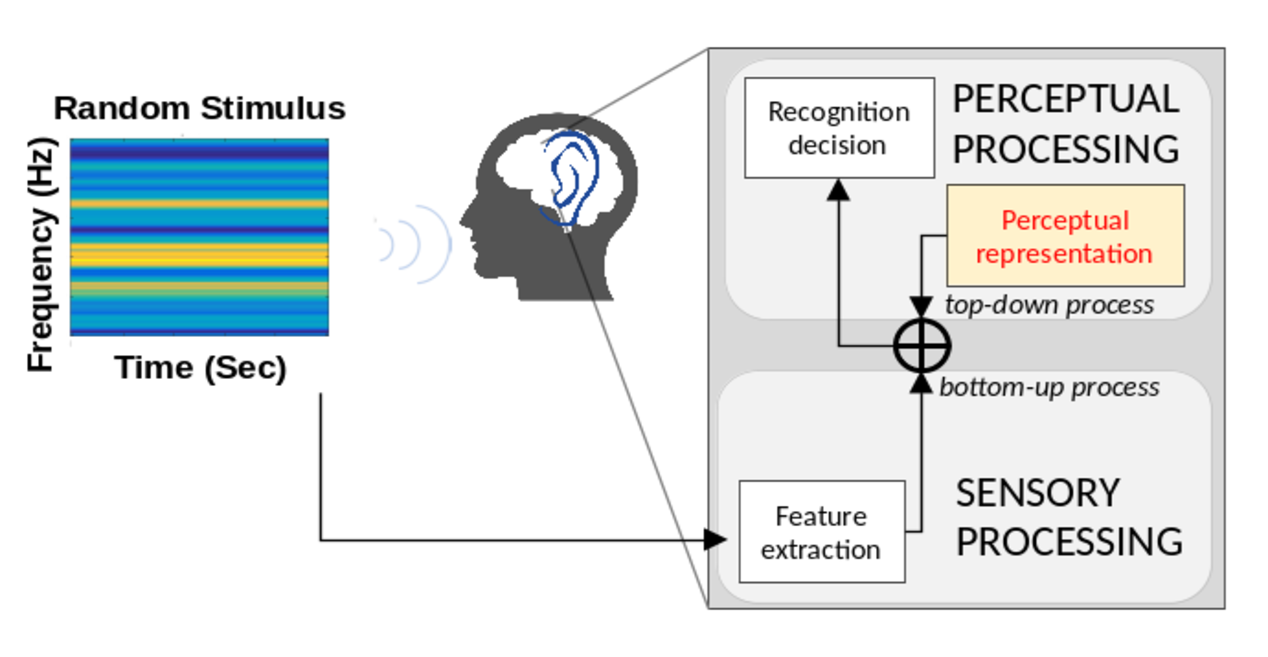
\includegraphics[width=0.8\textwidth]{Figures/Figures_tinnitus_1.png}
	\caption{Model of the discrimination task as a transductive process.
	Random stimuli is filtered by the subject using low-level sensory mechanisms.
	The perceptual discrimination task is modeled as a top-down process that
	compares the sensory information to a perceptual representation ``template''
	to determine if the stimulus belongs to that perceptual representation.}
	\label{fig:template}
\end{figure}

Reverse correlation has been applied across multiple fields to reveal underlying representations by application of unconstrained, noisy input.
It has been used to characterize low-level latent representations encapsulated in neural tuning
(\eg receptive fields) \cite{ringachReverseCorrelationNeurophysiology2004}
and has been used to successfully recover cognitive representations underlying visual perception \cite{gosselinSuperstitiousPerceptionsReveal2003,}
Both existing experimental work (\cf Fig 2B in \cite{brimijoinInternalRepresentationVowel2013})
and our preliminary simulation experiments (\autoref{fig:csexample}) suggest that this method can be successfully translated
into the auditory domain.
Reverse correlation allows us (\emph{a}) to uncover more complex, potentially higher-dimensional representations
than would be possible using more focused, constrained stimuli,
(\emph{b} to recover directly the nature of the representations themselves rather than the relation
between the tinnitus percept and a masking sound,
and (\emph{c}) to recover cognitive representations of the tinnitus percept directly rather than a neural correlate.
In short, reverse correlation will be able to provide deeper understanding of cognitive representations of tinnitus percepts
than is possible with conventional methods.

\subsubsection*{C.1. Method}

The proposed method for uncovering perceptual representations can be divided
into a sequence of three main parts:
(1) construction of vague, ``random'' stimuli for presentation to subjects,
(2) experimental procedure and data collection,
and (3) reconstruction of perceptual representations from subject responses.

% \begin{description}
% 	\item[C.1.1. Stimuli Construction]{}
% \end{description}

\paragraph{Stimuli construction}

Stimuli will be generated randomly, in keeping with prior work in the visual domain
\cite{gosselinSuperstitiousPerceptionsReveal2003}.
The meaning of ``random'' with respect to the stimuli presented to subjects
refers specifically to the shape of spectral envelope in the frequency domain.
This shape will be determined randomly for all stimuli
and will not be informed by prior knowledge
or statistics over canonical examples of tinnitus.
These random spectral envelopes will be used as the basis for building spectrograms
that sound like tinnitus percepts.

Our preliminary testing suggests that truly random envelopes
often result in the perception of colored noise.
Minimal additional spectral-temporal constraints may need to be imposed on stimuli
such that participants will interpret the stimuli as intending to be tinnitus percepts.
This is similar to the approach taken in some visual domain experiments,
where bandlimited random stimuli, or stimuli with partial superimposed templates,
are presented \cite{smithMeasuringInternalRepresentations2012}.
The basic approach will be to use inverse Fourier transforms to generate 0.5-s noise stimuli
including frequencies from 0.1 to 22 kHz \cite{brimijoinInternalRepresentationVowel2013}.
We will impose minimal constraints on the stimuli generation process,
in order to selectively generate stimuli approaching the heterogeneous samples of tinnitus percepts
provided by the American Tinnitus Association on their website \cite{Symptoms2015}.

\paragraph{Subject Recruitment}

Subjects will be recruited from the clinical population by \hl{our clinical collaborator}
and will be assessed by the Tinnitus Severity Scale,
which measures the negative impact tinnitus has on a subject's quality of life.
We will not screen for unilateral or bilateral tinnitus but will only include subjects
with primary (\ie subjective, not somatosensory) tinnitus.

\paragraph{Experimental procedure}

During the experiment, subjects will be asked to perform an computerized alternate forced-choice task,
selecting whether the presented stimulus sounds similar to their tinnitus percept or not.
They will be told that the stimuli are tinnitus-like sounds corrupted by noise
and that not all will sound like their tinnitus percept.
Each signal will be presented to subjects over headphones
at an audible level ($\approx 75$ dB SPL) after which
the subject will select either ``yes'' or ``no'' via keyboard presses.
The next trial will begin after a 500-ms pause.
Subjects will be asked to perform the task in 80-trial blocks with a rest period in-between.
We will ask subjects to perform 20 blocks at minimum, which should take about a half an hour.
Subjects can perform the task for more blocks at their choice,
and will be compensated for their participation.

\paragraph{Reconstructing representations}

We will reconstruct cognitive representations of tinnitus from the data
by taking the least-squares fit to the behavioral data
(\autoref{fig:experiment}).
This is equivalent to interpreting the cognitive representation
as a ``classification spectrogram''
generated by subtracting the average of the negative trials from the average of the positive trials
\cite{gosselinSuperstitiousPerceptionsReveal2003}.
We theorize that in the underlying transductive cognitive process,
that the classification spectrogram is used as a template vector
against which stimuli are compared in a linear matching model of response generation.
While we acknowledge that this reconstruction approach is inefficient,
requiring many samples to acquire a coherent reconstruction,
it is well-studied in the literature
and will serve as a baseline against which our efficient reconstruction
algorithm in Aim \#2 will be compared.

\begin{figure}[h] % Figure at bottom of the page ([b] argument, could be "t" for top or "h" for here)
	\centering
	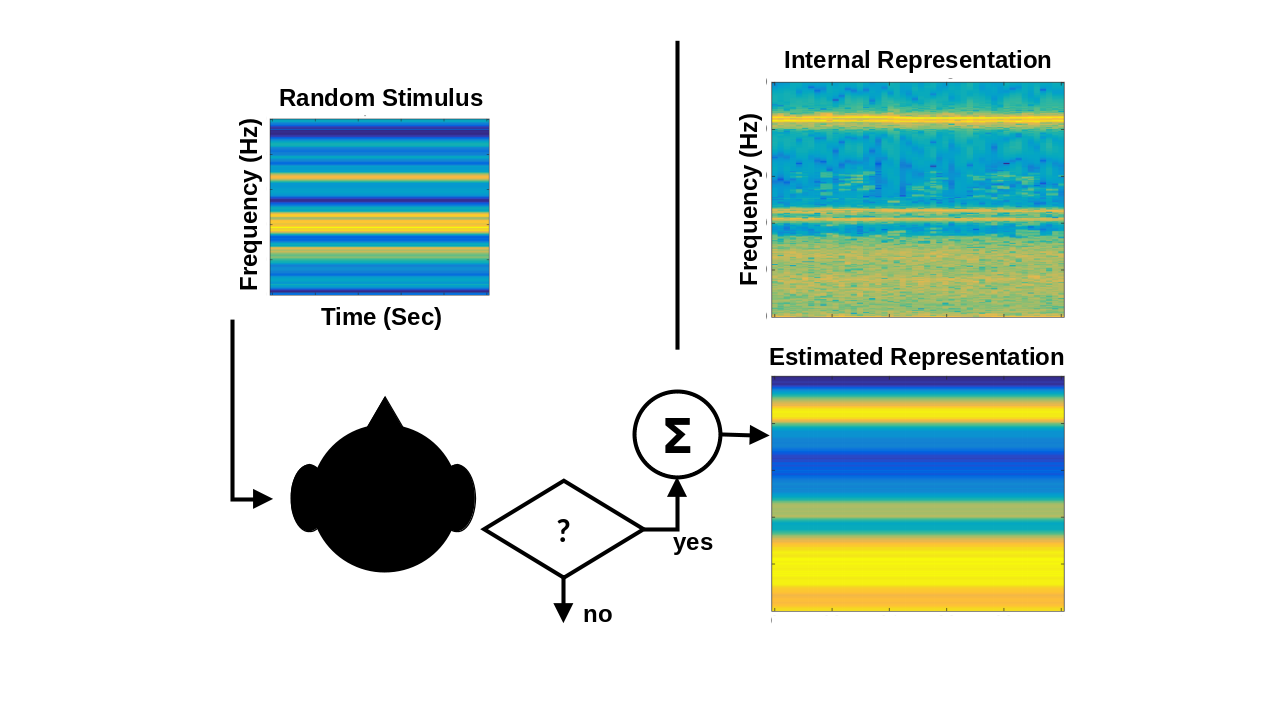
\includegraphics[width=0.8\textwidth]{Figures/Figures_tinnitus_3.png}
	\caption{Schematic overview of experiments proposed in Aim \#1.
	Subjects are presented with random stimuli,
	which is compared to a latent internal representation.
	Reverse correlation is used to reconstruct an estimate of the latent internal representation
	over many trials.
	Simulation results are shown, demonstrating proof-of-concept
	for the proposed reverse correlation paradigm.}
	\label{fig:experiment}
\end{figure}

\subsection*{C.2. Aim \#2: Develop an efficient reconstruction algorithm for cognitive representations using compressive sensing}

In this aim, we employ advanced signal processing techniques to overcome critical inefficiencies
in reverse correlation that limit its scope and impact.

Current attempts to characterize perceptual mechanisms using reverse correlation
are limited in scope due to inefficiencies inherent to conventional methods.
While reverse correlation allows for relatively unconstrained and unbiased
estimation of latent representations using straightforward stimulus-response data
\cite{marmarelisWhiteNoiseMethodSystem1978,nishimotoReceptiveFieldProperties2006},
the number of stimulus-response samples required for accurate estimation
is typically very large \cite{mineaultImprovedClassificationImages2009}.
This inefficiency limits the feasibility of applying reverse correlation more broadly,
as subject participation must be maintained over long timelines.

The impact of this inefficiency extends well beyond the present proposal.
This fundamental sampling problem affects similar efforts to estimate higher-level
cognitive representations and psychophysical kernels that drive top-down processes of perception
\cite{ahumadaStimulusFeaturesSignal1971,neriReceptivePerceptiveFields2006,gosselinSuperstitiousPerceptionsReveal2003,smithMeasuringInternalRepresentations2012}.
Since reverse correlation has broad applicability for characterizing any aspect
of neurological, cognitive, or psychological function that can be modeled as a transductive process
\cite{ringachReverseCorrelationNeurophysiology2004},
the inefficiencies of reverse correlation impact efforts
to characterize phenomena as fine-grained as latent neural representations (\eg neural receptive fields) \cite{ringachReverseCorrelationNeurophysiology2004}
and as high-level  as abstract psychological categories (\eg ``male'' vs. ``female'' faces)
\cite{brinkmanVisualisingMentalRepresentations2017,ponsotCrackingSocialCode2018,manginiMakingIneffableExplicit2004}.
To combat this efficiency limitation, studies often 
(\emph{a}) limit the richness of the stimuli (\eg by only allowing specific aspects of the stimulus to vary)
\cite{gosselinBubblesTechniqueReveal2001},
or (\emph{b}) impose some constraints on the inferred representations,
for instance by smoothing the raw estimates \cite{gosselinSuperstitiousPerceptionsReveal2003}.
The constraints imposed by these approaches ultimately defeat the full power of reverse correlation
\cite{murrayTroublesBubbles2004},
leading to estimates that are biased or incomplete.

We propose to develop an advanced signal processing pipeline
that will enable us to overcome the inefficiencies of existing reverse correlation methods
through the use of \emph{compressive sensing},
a recent advance in signal processing which has led to dramatic improvements in efficiency
over conventional sampling and signal estimation methods
\cite{baraniukCompressiveSensingLecture2007}.
Compressive sensing has recently gain wide recognition in domains such as medical imaging
\cite{graffCompressiveSensingMedical2015,lustigCompressedSensingMRI2008},
where considerations of efficiency and bias reduction are critical.
Compressive sensing holds promise to similarly improve the efficiency of reverse correlation
without the drawback of biasing estimates.
Compressive sensing will extend the range of possible cognitive and perceptual mechanisms that can be estimated
by dramatically decreases the number of trials needed for signal reconstruction.
Since compressive sensing can be directly substituted for conventional, regression-based estimation,
it can be directly substituted into existing experimental protocols without requiring other changes.
Our ultimate objective is to develop and validate a compressive sensing
data processing pipeline – culminating in an open-source software tool – that will allow for
efficient and accurate reconstruction of latent representations using data 
obtained via the reverse correlation method.

\paragraph{Compressive sensing framework}

Many natural signals, $x$, including latent representations, are compressible,
meaning that they can be represented by a sum of a small number of functions
from an appropriately-chosen basis set ($s = \Psi^{T}x$, for basis $\Psi$ and weights $s$).
A key insight of compressive sensing is that response variables, $y$,
stem from a process of comparing stimuli to latent representations
($y = \Phi x$, for measurement $\Phi$) (\autoref{fig:csexplanation}).
It is then possible to estimate the latent representation
using only a small number of measurements
by acquiring the basis function representation directly (\ie $ y = \Phi \Psi s$)
via sparse optimization (to find $s$).
The responses can be continuous (\eg firing rates),
ordinal similarity scores
\cite{zymnisCompressedSensingQuantized2010},
or binary \cite{boufounos1BitCompressiveSensing2008,planOneBitCompressedSensing2013},
as in the proposed experiments here.
In practice, sparse representations can be found even when the chosen basis domain is quite general
and incorporates no prior knowledge of the signal's characteristics
(\eg the discrete cosine transform or wavelet transform).
Critically, it has been shown that using random stimuli to elicit
and subsequently observe responses
is a highly effective way to ensure accurate reconstruction of latent representations
within the compressive sensing framework
\cite{candesIntroductionCompressiveSampling2008,candesRestrictedIsometryProperty2008,wojtaszczykStabilityInstanceOptimality2010}.
In other words, the somewhat
unusual model of sampling assumed by compressive sensing maps directly onto reverse correlation.

\begin{figure}[h] % Figure at bottom of the page ([b] argument, could be "t" for top or "h" for here)
	\centering
	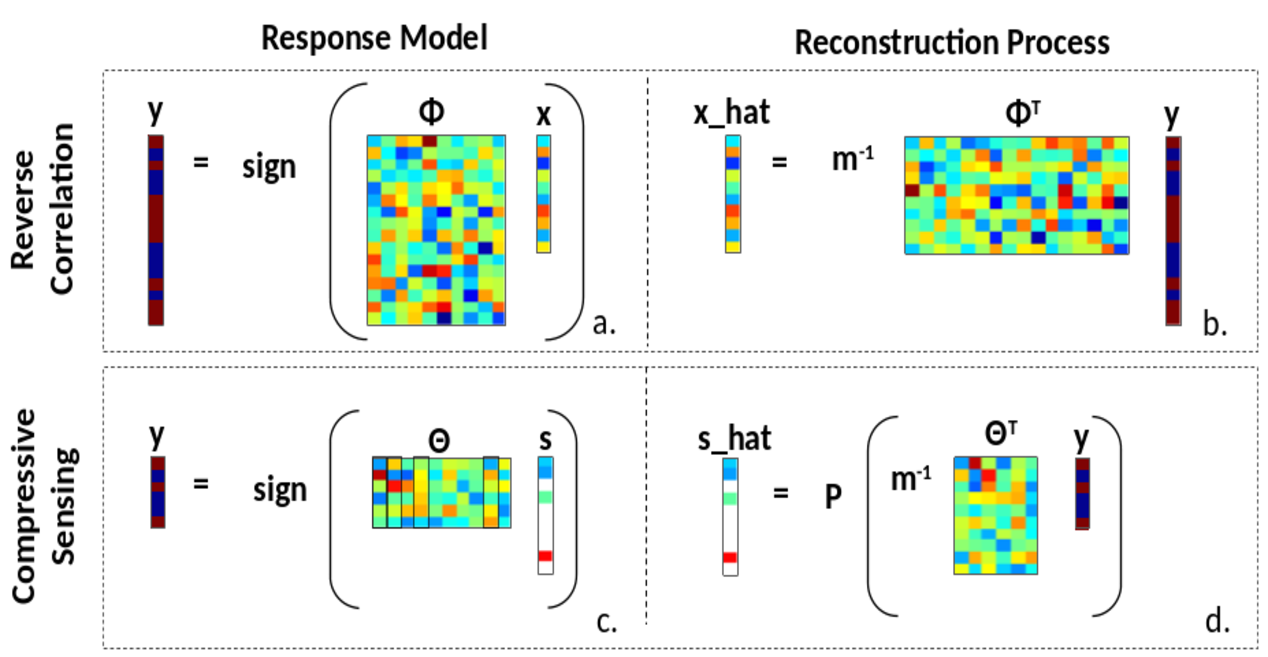
\includegraphics[width=0.8\textwidth]{Figures/Figures_tinnitus_5.png}
	\caption{Comparison of reverse correlation and compressive sensing.
	(\emph{a}) In reverse correlation, the vector of subject responses is modeled as
	resulting from the multiplication of a latent representation vector, $x$,
	and a stimulus matrix, $\Phi$, which can be thought of as a similarity calculation
	between the latent representation and a vector representation of each presented stimulus.
	(\emph{b}) An estimate of the latent representation, $\hat{x}$, is then reconstructed
	by regressing responses against the stimuli.
	(\emph{c}) In compressive sensing,
	the vector of subject responses is modeled as resulting from the multiplication
	of a sparse latent representation vector, $s$, and a compressive sensing matrix, $\Theta$.
	The compressive sensing matrix is formed by multiplying a matrix of basis functions
	by the stimulus matrix, $\Theta = \Phi \Psi$, which amounts to a similarity calculation
	between the stimuli and the known basis functions.
	(\emph{d}) An estimate of the sparse latent representation, $\hat{s}$, is then reconstructed
	by regressing the responses against the compressive sensing sparse representations
	and known basis functions, $\hat{x} = \Psi \hat{s}$. Note that the response vector, $y$,
	in compressive sensing is generally assumed to contain many fewer entries than
	in reverse correlation without sacrificing reconstruction accuracy.}
	\label{fig:csexplanation}
\end{figure}

\paragraph{Simulations and preliminary evidence}

We have conducted simulation studies to begin validating compressive sensing
for improving the efficiency of reverse correlation.
For example, using a template time-frequency representation, $x$,
as a proxy for the latent representation of interest,
we generate plausible yes/no subject responses, $y \in \{-1, 1\})$,
based on the similarity between the template
and a random stimuli (\ie $y = \mathrm{sign}(\phi x)$ for stimuli $\phi$).
Estimation of the template is performed using
(\emph{a}) convention regression-based reverse correlation
(\ie $\hat{x}_c = n^{-1} X^\mathrm{T}y$) \cite{gosselinSuperstitiousPerceptionsReveal2003},
or (\emph{b}) compressive sensing.

\autoref{fig:csexample} shows example results from our preliminary simulation studies.
In this example, we attempt to reconstruct a spectrally-rich signal.
Four reconstructions are shown, corresponding to two sample sizes (12,500 and 100,000 samples)
and two reconstruction methods (conventional linear regression and compressive sensing).
The signal quality obtained using fewer samples via compressive sensing
is effectively equivalent to that obtained using eight times more samples
via conventional reconstruction.
When allowed to operate on the full complement of 100,000 samples,
compressive sensing shows +21\% improved accuracy over conventional reconstruction.
If further simulation studies and validation on real data continue to align with these preliminary results,
the number of trials required for accurate estimation using reverse correlation paradigms
could be reduced to 12.5\% of the current standard.
Such a drastic increase in time- and cost-effectiveness would substantially
increase the method's potential for widespread use.

\begin{figure}[h] % Figure at bottom of the page ([b] argument, could be "t" for top or "h" for here)
	\centering
	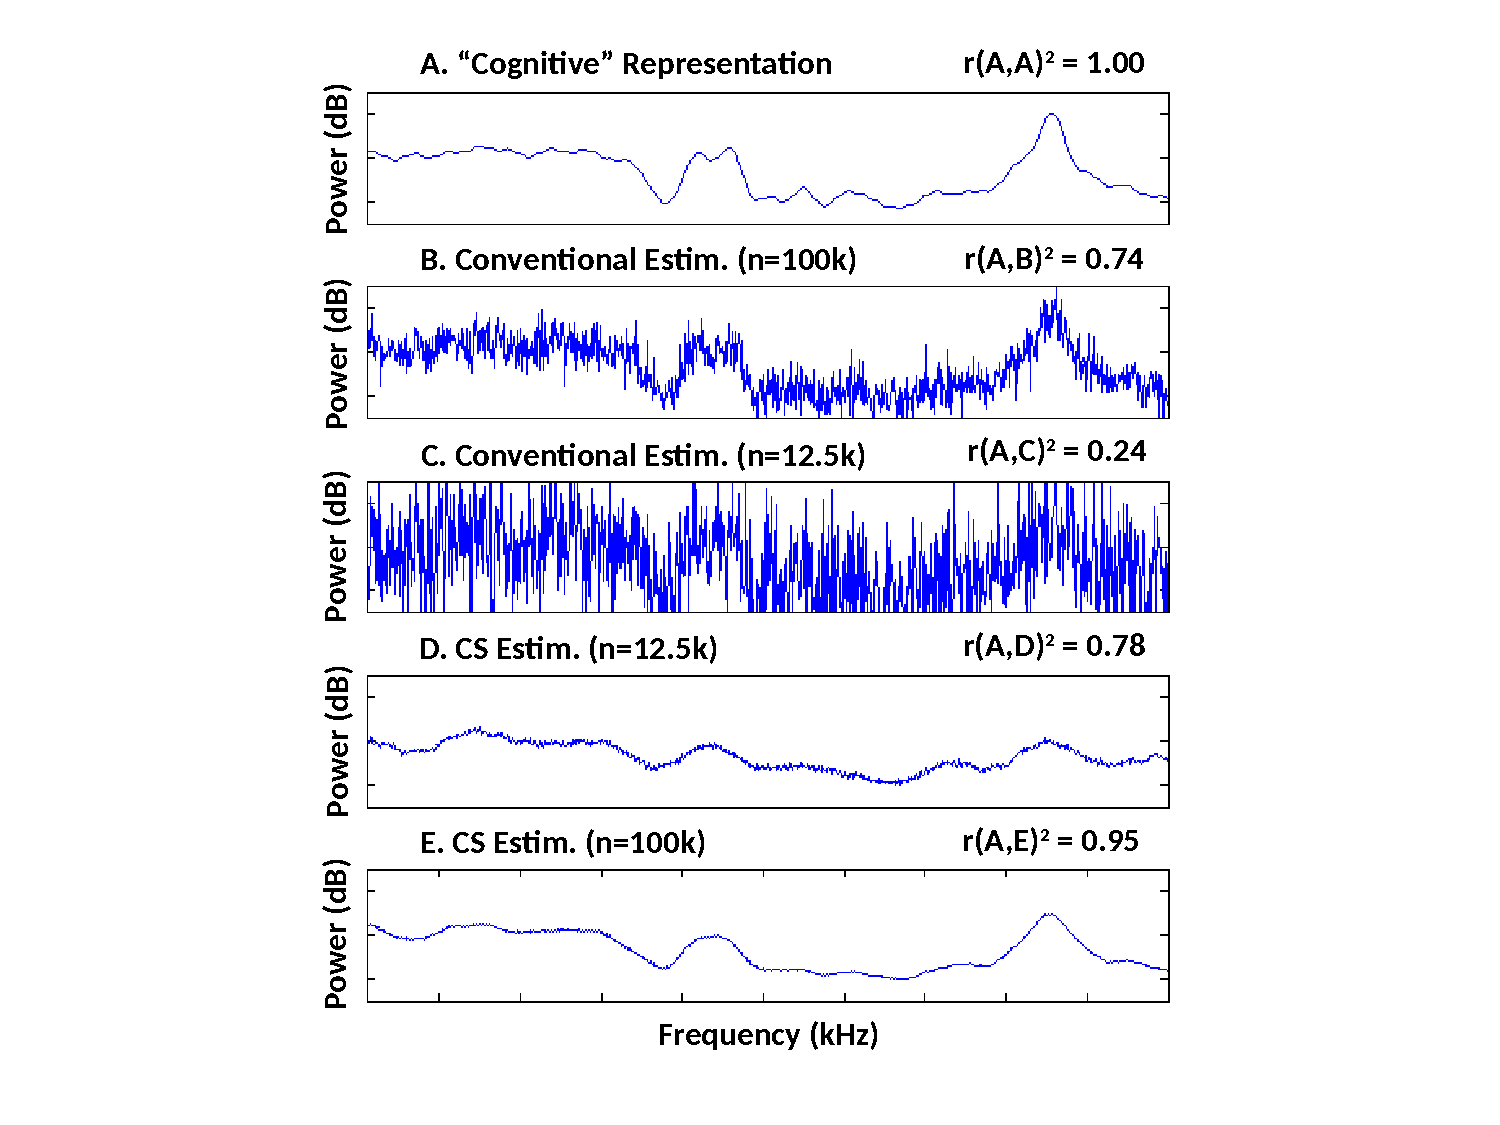
\includegraphics[width=\textwidth]{Figures/CompSensExamples.pdf}
	\caption{Compressive sensing (CS) delivers accurate signal reconstruction from sampling
	with a comparatively small number of samples.
	The latent representation in (\emph{A}) is estimated in (\emph{B-E}).
	In (\emph{B-C}) conventional regression-based estimation is used
	and in (\emph{D-E}) compressive sensing is used.
	The number of samples, $n$, is displayed along with the correlation coefficient, $r^2$,
	between the estimated reconstruction and the original signal,
	as a measure of reconstruction quality.}
	\label{fig:csexample}
\end{figure}

\paragraph{Validation of compressive sensing}

We will validate the proposed use of compressive sensing for relevant
cognitive and behavioral data.
Validation will be accomplished through simulation studies
(\eg expanding on the simulation results discussed herein)
and through analysis of data collected in Aim \#1.
We will assess outcomes by examining estimation performance
as a function of sample size,
incuding
(\emph{a}) reconstruction accuracy with few samples,
(\emph{b}) gains in high-sample reconstruction accuracy, and
(\emph{c}) minimal sample size to achieve high-end convergent accuracy.
The basis for these assessments will be a comparison
with the conventional, full-sample reconstruction
as described in Aim \#1,
since the true gold standard representation is unavailable.
Potential improvements of compressive sensing reconstruction
will be assessed using signal quality metrics that do not require direct comparison
(\eg peak signal-to-noise ratio).
This work will determine optimal parameters for compressive sensing
in tinnitus percept reconstruction.
We expect these parameters to depend on stimulus type, response noise,
and the type of tinnitus experienced by the subject.
Considered parameters will include appropriate input/output representations,
reconstruction algorithm, and basis type/sparsity.

\paragraph{Development of an open-source software tool}

We will develop and distribute an open-source software tool for conducting
auditory perceptual experiments using reverse correlation,
including stimulus presentation, response collection,
and representation reconstruction, characterization, and comparison
as described in Aim \#3.
This software package will include both standard reconstruction methods
as well as an implementation of the compressive sensing framework,
informed by the findings in this Aim, for use by the research community.
We will develop interfaces for widely-used programming languages
(including MATLAB and Python) in addition to command-line executables.
Making the platform open-source provides opportunities for the community
to make improvements and enables researchers to tailor these methods to their specific use-cases.

Reverse correlation has the potential to uncover latent representations underlying perception, and
transform our understanding of perceptual mechanisms at various levels of investigation: neural, cognitive
and psychological. However, in order for this potential to be fully realized, the fundamental inefficiency of
reverse correlation paradigms must be overcome. Compressive sensing holds promise to overcome this
limitation by dramatically improving the efficiency of reverse correlation, enabling its extension to
perceptual mechanisms that are out of reach using current methods. The work proposed here will enable
researchers to access the promise of compressive sensing, broadening the impact of reverse correlation.

\subsection*{C.3. Aim \#3: Characterize and interpret cognitive representations of tinnitus}

Our approach in this goal is to characterize the properties of uncovered representations
through computational modeling.
In Aim \#1, we will have collected tinnitus percept data using the reverse correlation method.
In Aim \#2, we will have reconstructed high-dimensional representations of tinnitus percepts
using both conventional and compressive sensing methods.
In this Aim, we will characterize the space of representations
to investigate correspondence between data-driven subtypes and qualitative subtypes,
evaluate the stability of tinnitus percepts over time,
and accelerate the diagnostic process.

\paragraph{Data-driven tinnitus subtypes}

Surveys of tinnitus patients have identified sixteen qualitative subtypes of tinnitus
\cite{vajsakovicPrinciplesMethodsPsychoacoustic2021,meikleTinnitusArchiveArchive2004,stoufferCharacterizationTinnitusTinnitus1990},
but these categories are limited by the fuzziness of linguistic categories and the musical ability of the tinnitus patients.
Tinnitus subtypes are used to better explain and quantify the condition,
however qualitative subtypes are ill-defined.
While one tinnitus patient we interviewed, who has a degree in music performance,
was able to identify her tinnitus as sounding like a particular note played on the crotales,
a niche percussion instrument,
most tinnitus patients lack the depth of vocabulary to explain their tinnitus percept that precisely.
Accordingly, linguistic description of tinnitus can be vague and overlapping.
For instance, two of the subtypes in \cite{vajsakovicPrinciplesMethodsPsychoacoustic2021} are ``high tension wire'' and ``transformer noise.''
Is ``high tension wire'' meant in the colloquial sense of high-voltage power lines,
or does it mean the reverberation of a tightly-pulled string?
If the latter, then how is the sound of a high-voltage power line
disambiguated from the sound of a distribution transformer,
which is
mounted on a utility pole and connected directly to the high-voltage wires?
Instead of linguistic categories, we propose to use latent variable analysis
to reveal data-driven subtypes of tinnitus.

We will perform a quantitative analysis of tinnitus representations based on latent variable analysis methods
to reveal underlying similarities between representations.
Latent variable methods relate observed variation (\eg in tinnitus representations)
to latent variables that capture the observed variation (\eg major variation types across tinnitus percepts).
We will use principle component analysis (PCA) and uniform manifold approximation and projection (UMAP; \cite{mcinnesUMAPUniformManifold2020}).
Applying these dimensionality-reduction algorithms to a collection of representations
will identify major modes of variation across those representations,
uncovering latent similarities between representations.
Clusters of data points become readily visible in the lower-dimensional manifold generated
by these unsupervised machine learning methods, each of which represents
a data-driven tinnitus subtype (\autoref{fig:dimredexample}).
We will characterize these subtypes, identifying their properties and assigning them descriptive names.
New data can be mapped into the lower-dimensional manifold,
allowing representations from new subjects to be classified into these subtypes.

\begin{figure}[h] % Figure at bottom of the page ([b] argument, could be "t" for top or "h" for here)
	\centering
	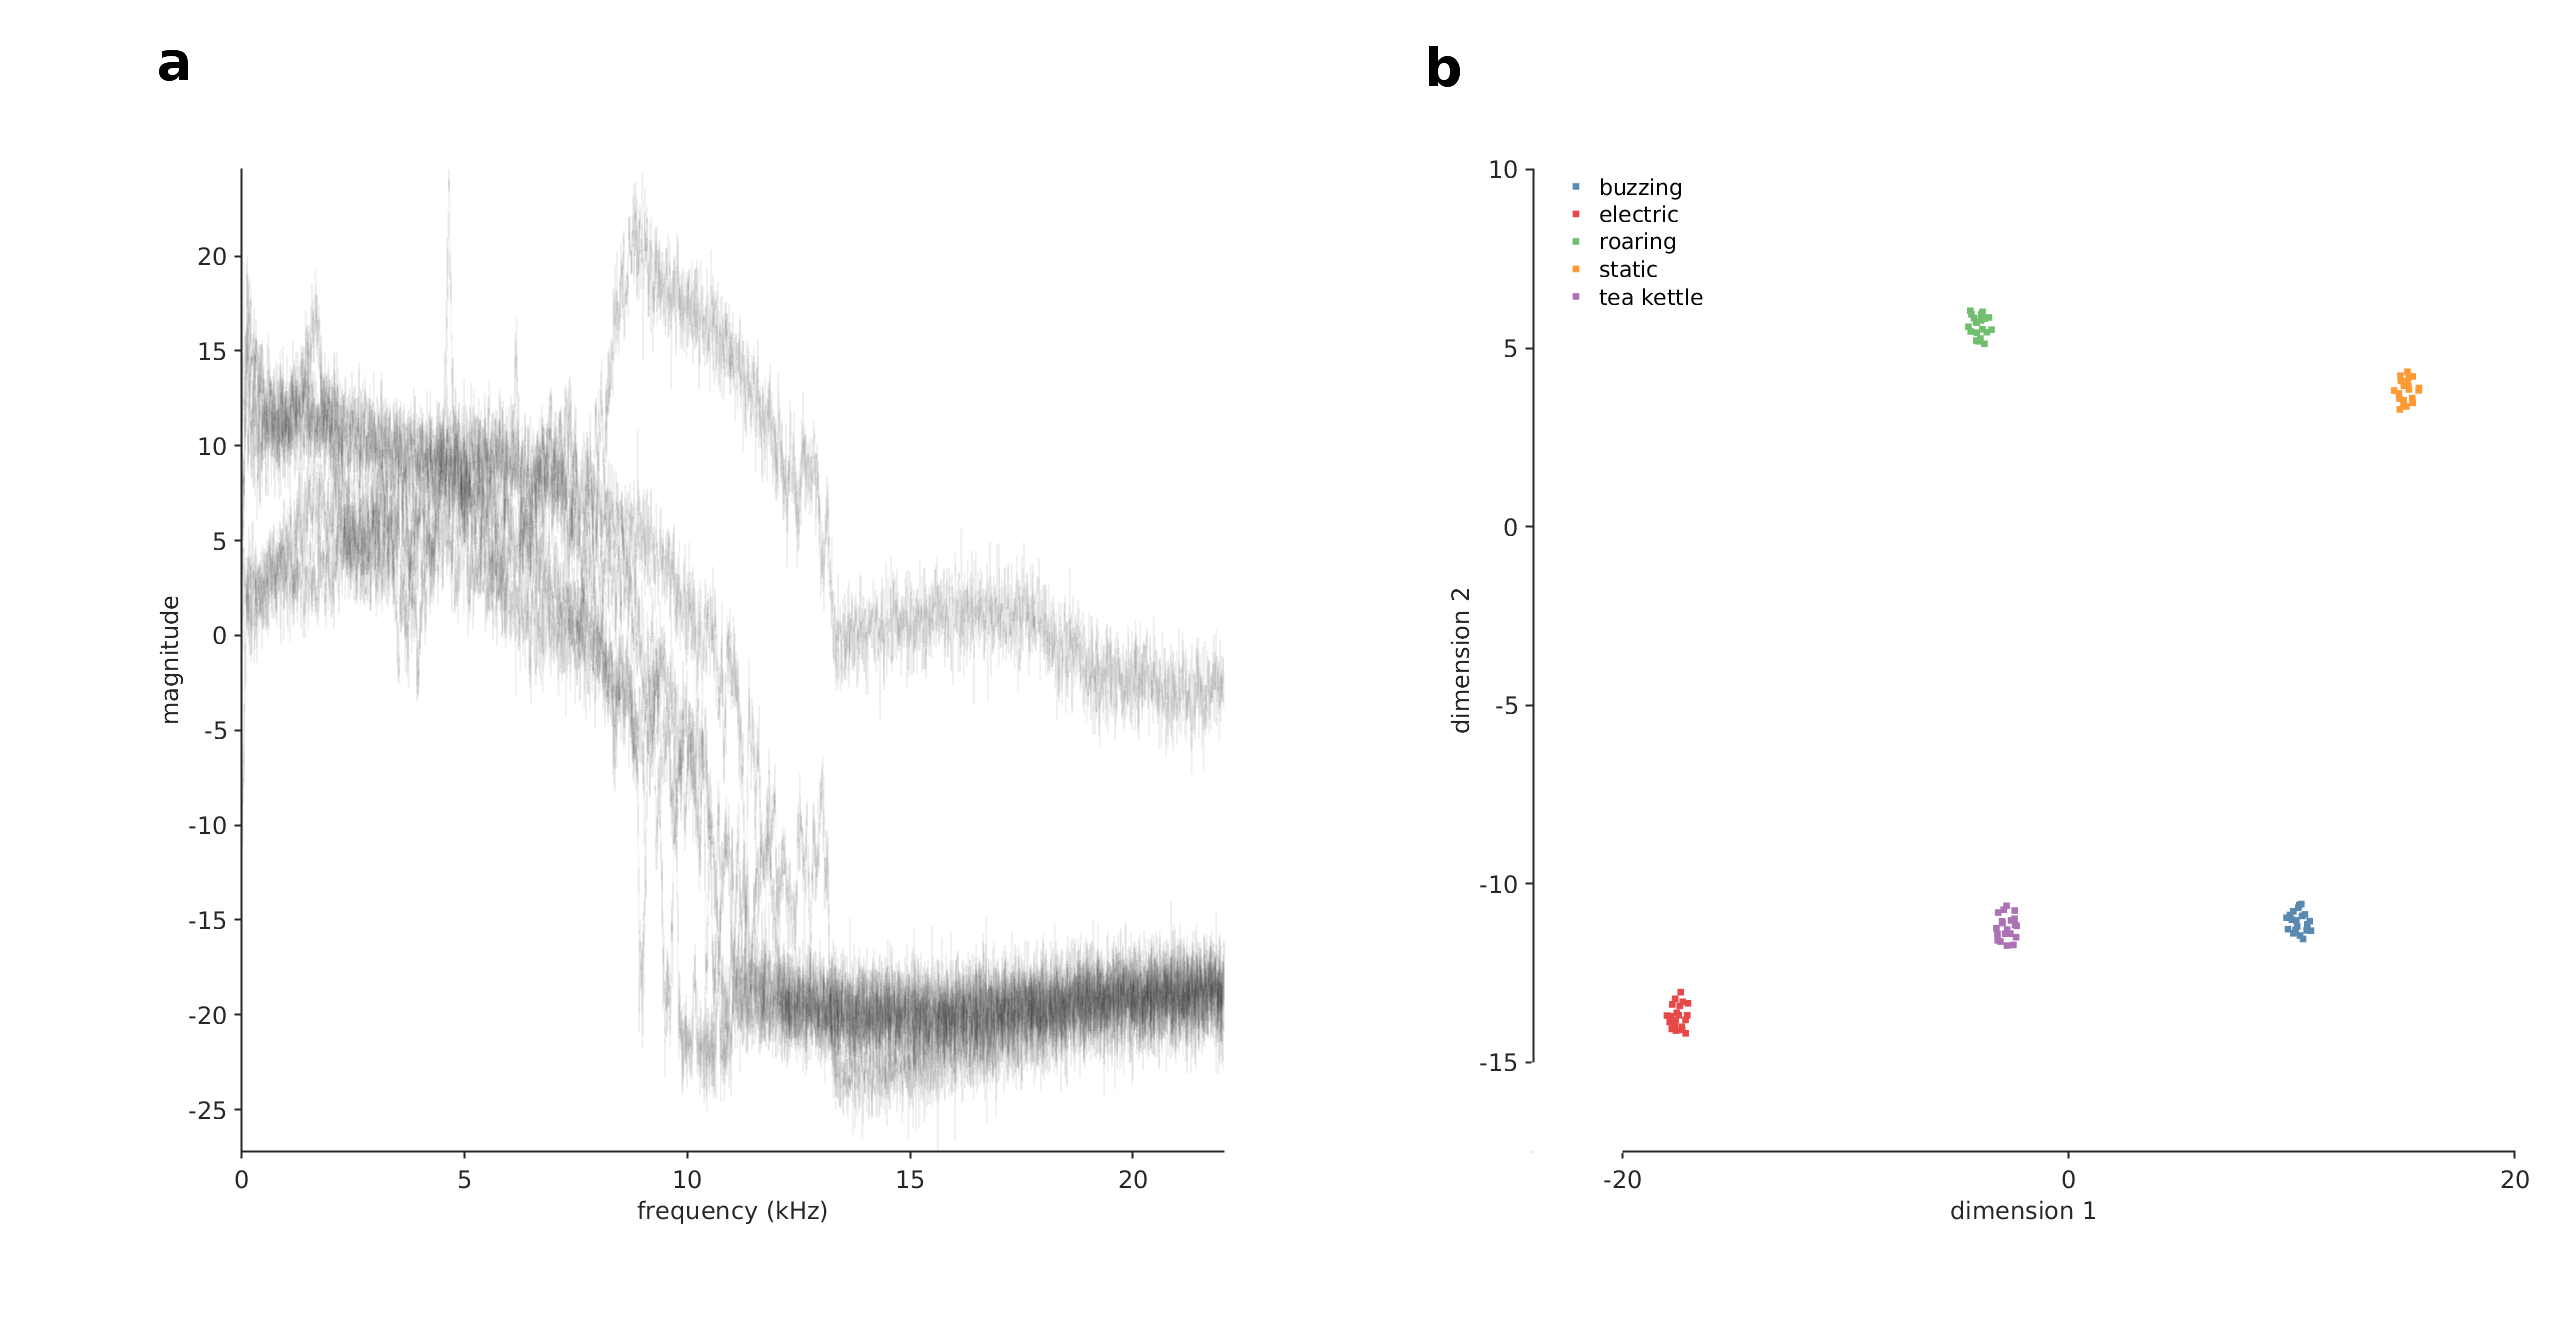
\includegraphics[width=0.8\textwidth]{Figures/umap.png}
	\caption{Tinnitus representations with different spectral characteristics cluster in a lower dimensional manifold.
	Tinnitus representation waveforms were generated
	using examples from the American Tinnitus Association website with added Gaussian noise
	\cite{Symptoms2015}.
	(\emph{a}) shows the frequency spectra for representative waveforms. (\emph{b}) The waveforms
	are dimensonally-reduced using UMAP from 8,193 dimensions to 2.
	The waveforms cluster in this lower dimensional space, revealing latent similarities.}
	\label{fig:dimredexample}
\end{figure}

\paragraph{Improving stimuli generation through data-driven distributions}

In Aim \#1, we generate stimuli by randomly sampling Fourier coefficients from a flat distribution to generate a spectrum.
We enforce only minimal constraints on the stimuli (\eg that the frequency content is audible).
This has the benefit of reducing bias in the reconstructed representations,
but results in experiments that take longer to converge to a good reconstruction.
Previous studies using reverse correlation have attempted to reduce noise in the reconstructed representation
(and thus converge much faster) by carefully selecting stimuli biased towards a certain representation.
For example, Smith and colleagues \cite{smithMeasuringInternalRepresentations2012}
devised a task to uncover cognitive representations of faces using reverse correlation,
using pictures of human faces distorted by noise as stimuli for the task.
While this allowed the experimenters to perform fewer trials to achieve good reconstructions,
it introduced bias of what experimenters think human faces look like (by selecting the pictures),
defeating one of the main advantages of reverse correlation.

We propose to improve stimuli generation by exploiting our data from subsequent experiments.
Each putative reconstruction that we uncover leads to a new known data point hypothesized to lie on the manifold
of tinnitus representations.
We can treat this manifold much like a distribution and sample our stimuli from it,
resulting in stimuli that sound ``less random'' and more like actual tinnitus percepts.
This closed-loop experimental protocol means that our stimuli generation becomes more tinnitus-like
with every reconstruction, without introducing experimenter bias \emph{a priori}.

We will implement a variational autoencoder (VAE), a type of unsupervised machine learning model
that learns a latent representation of data as well as how to generate new data
that appears similar to data the model has been presented with before.
A VAE consists of an encoder artificial neural network
which constructs a latent representation
as a zero-mean, unit-variance normal-distributed vector
and a decoder artificial neural network
that reconstructs the input (\autoref{fig:vae}).
By training the VAE on reconstructed representations,
forcing the encoder to create a latent representation
and the decoder to reproduce the input from the latent representation,
the model will learn the manifold of tinnitus percepts.
By sampling the latent vector,
we can generate new stimuli informed by the representations the model has learned.
One limitation of VAEs is that sampling from the latent distribution
tends to produce new data points that appear noisy.
In our experiment, this is a benefit,
as noisy, random stimuli is crucial to reverse correlation.
Through this generative model,
we will create stimuli that appear closer to actual tinnitus percepts
by learning directly from the data
without introducing external experimenter bias.

\begin{figure}[h] % Figure at bottom of the page ([b] argument, could be "t" for top or "h" for here)
	\centering
	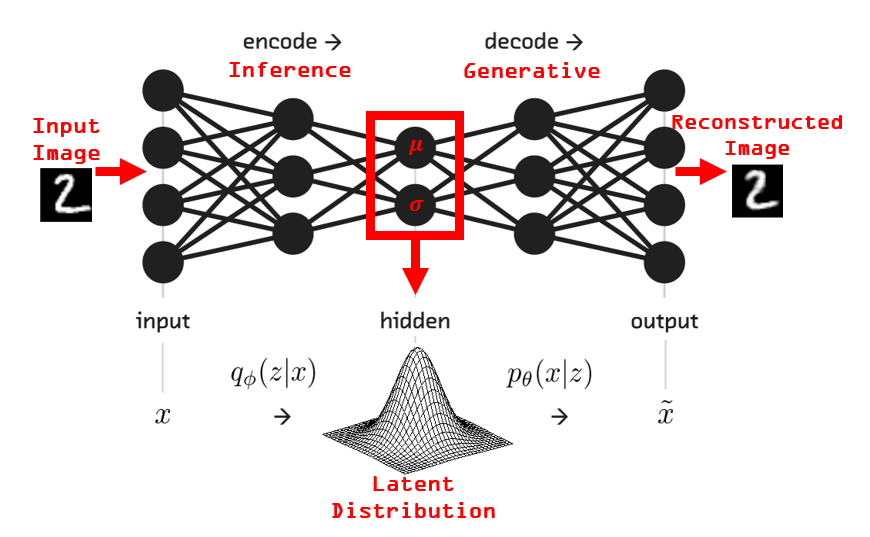
\includegraphics[width=0.8\textwidth]{Figures/variational-autoencoder.png}
	\caption{Diagram of a variational autoencoder (VAE) learning a representation of the digit ``2''.
	VAEs assume that the data, $x$, are generated by a directed graphical model, $p_\theta(x|z)$,
	and that the encoder is learning an approximation $q_\phi(z|x)$, where $\phi$ and $\theta$
	denote the parameters of encoder and decoder respectively.
	The latent representation, $z$, is interpreted as originating from a multivariate Gaussian distribution.
	By sampling from the latent distribution, new data can be generated. Figure from \cite{IntroductionAutoencoders2020}.}
	\label{fig:vae}
\end{figure}

\paragraph{Acceleration of diagnosis through subtype identification}

While we anticipate remarkable performance gains in the number of samples required for accurate representation
through compressive sensing,
it may be clinically useful to identify only the subtype of tinnitus
(\ie which cluster on the lower-dimensional manifold the representation belongs to)
to some convergent accuracy.
If only the subtype is needed,
we believe the number of samples required for convergent accuracy can be further reduced.
We will devise an algorithm to perform the data-driven tinnitus subtyping ``online''
while the subject performs the task.
When convergent accuracy is reached, the task will automatically conclude.
By this process, both patient and clinician time is optimized, while still providing high-fidelity quantitative medical data
for use in diagnosis and treatment.

\paragraph{Stability of tinnitus percepts over time}

It is an open question in tinnitus research, whether tinnitus percepts remain stable over time
\cite{husainReplicabilityNeuralBehavioral2019}.
Using data from subjects who returned to perform the experiment multiple times
over the course of several weeks,
we will examine representations derived from each experiment instance
to quantitatively evaluate drift in the tinnitus representation over time.
We will assess measures of variance and spectral distance between representations
computed during different temporally-separated experiment sessions.

% %----------------------------------------------------------------------------------------
% %	PROGRESS REPORT
% %----------------------------------------------------------------------------------------

% \newpage

% \section*{5. Progress Report Publication List (Renewal Applications Only)}

% List the titles and complete references to all appropriate publications, manuscripts accepted for publication, patents, and other printed materials that have resulted from the project since it was last reviewed competitively. When citing articles that fall under the Public Access Policy, were authored or co-authored by the applicant and arose from NIH support, provide the NIH Manuscript Submission reference number (e.g., NIHMS97531) or the Pubmed Central (PMC) reference number (e.g., PMCID234567) for each article. If the PMCID is not yet available because the Journal submits articles directly to PMC on behalf of their authors, indicate "PMC Journal -- In Process." A list of these journals is posted at: http://publicaccess.nih.gov/submit\_process\_journals.htm.

% Citations that are not covered by the Public Access Policy, but are publicly available in a free, online format may include URLs or PMCID numbers along with the full reference (note that copies of these publications are not accepted as appendix material, see Part I Section 5.5.15 for more information).

% %----------------------------------------------------------------------------------------
% %	PROTECTION OF HUMAN SUBJECTS
% %----------------------------------------------------------------------------------------

% \newpage

% \section*{6. Protection of Human Subjects}

% Refer to Part II, Supplemental Instructions for Preparing the Human Subjects Section of the Research Plan.

% This section is required for applicants answering "yes" to the question "Are human subjects involved?" on the R\&R Other Project Information form. If the answer is "No" to the question but the proposed research involves human specimens and/or data from subjects applicants must provide a justification in this section for the claim that no human subjects are involved.

% Do not use the protection of human subjects section to circumvent the page limits of the Research Strategy.

% %----------------------------------------------------------------------------------------
% %	INCLUSION OF WOMEN AND MINORITIES
% %----------------------------------------------------------------------------------------

% \newpage

% \section*{7. Inclusion of Women and Minorities}

% Refer to Part II, Supplemental Instructions for Preparing the Human Subjects Section of the Research Plan. This section is required for applicants answering "yes" to the question "Are human subjects involved?" on the R\&R Other Project Information form and the research does not fall under Exemption 4.

% %----------------------------------------------------------------------------------------
% %	INCLUSION OF CHILDREN
% %----------------------------------------------------------------------------------------

% \newpage

% %\section*{8. Targeted/Planned Enrollment} - form to fill out 
% \section*{9. Inclusion of Children}

% Refer to Supplemental Instructions for Preparing the Human Subjects Section of the Research Plan, Sections 4.4 and 5.7. For applicants answering "Yes" to the question "Are human subjects involved" on the R\&R Other Project Information Form and the research does not fall under Section 4, this section is required.

% %----------------------------------------------------------------------------------------
% %	VERTEBRATE ANIMALS
% %----------------------------------------------------------------------------------------

% \newpage

% \section*{10. Vertebrate Animals}

% If Vertebrate Animals are involved in the project, address each of the five points below. This section should be a concise, complete description of the animals and proposed procedures. While additional details may be included in the Research Strategy, the responses to the five required points below must be cohesive and include sufficient detail to allow evaluation by peer reviewers and NIH staff. If all or part of the proposed research involving vertebrate animals will take place at alternate sites (such as project/performance or collaborating site(s)), identify those sites and describe the activities at those locations. Although no specific page limitation applies to this section of the application, be succinct. Failure to address the following five points will result in the application being designated as incomplete and will be grounds for the PHS to defer the application from the peer review round. Alternatively, the application’s impact/priority score may be negatively affected.

% If the involvement of animals is indefinite, provide an explanation and indicate when it is anticipated that animals will be used. If an award is made, prior to the involvement of animals the grantee must submit to the NIH awarding office detailed information as required in points 1-5 above and verification of IACUC approval. If the grantee does not have an Animal Welfare Assurance then an appropriate Assurance will be required (See Part III, Section 2.2 Vertebrate Animals for more information).
% The five points are as follows:

% \begin{enumerate}
% 	\item Provide a detailed description of the proposed use of the animals in the work outlined in the Research Strategy section. Identify the species, strains, ages, sex, and numbers of animals to be used in the proposed work.
% 	\item Justify the use of animals, the choice of species, and the numbers to be used. If animals are in short supply, costly, or to be used in large numbers, provide an additional rationale for their selection and numbers.
% 	\item Provide information on the veterinary care of the animals involved.
% 	\item Describe the procedures for ensuring that discomfort, distress, pain, and injury will be limited to that which is unavoidable in the conduct of scientifically sound research. Describe the use of analgesic, anesthetic, and tranquilizing drugs and/or comfortable restraining devices, where appropriate, to minimize discomfort, distress, pain, and injury.
% 	\item Describe any method of euthanasia to be used and the reasons for its selection. State whether this method is consistent with the recommendations of the American Veterinary Medical Association (AVMA) Guidelines on Euthanasia. If not, include a scientific justification for not following the recommendations.
% \end{enumerate}

% Do not use the vertebrate animal section to circumvent the page limits of the Research Strategy.

% %----------------------------------------------------------------------------------------
% %	SELECT AGENT RESEARCH
% %----------------------------------------------------------------------------------------

% \newpage

% \section*{11. Select Agent Research}

% Select Agents are hazardous biological agents and toxins that have been identified by DHHS or USDA as having the potential to pose a severe threat to public health and safety, to animal and plant health, or to animal and plant products. CDC maintains a list of these agents. See http://www.cdc.gov/od/sap/docs/salist.pdf.

% %----------------------------------------------------------------------------------------
% %	MULTIPLE PD/PI LEADERSHIP PLAN
% %----------------------------------------------------------------------------------------

% \newpage

% \section*{12. Multiple PD/PI Leadership Plan}

% For applications designating multiple PD/PIs, a leadership plan must be included. A rationale for choosing a multiple PD/PI approach should be described. The governance and organizational structure of the leadership team and the research project should be described, including communication plans, process for making decisions on scientific direction, and procedures for resolving conflicts. The roles and administrative, technical, and scientific responsibilities for the project or program should be delineated for the PD/PIs and other collaborators.

% If budget allocation is planned, the distribution of resources to specific components of the project or the individual PD/PIs should be delineated in the Leadership Plan. In the event of an award, the requested allocations may be reflected in a footnote on the Notice of Grant Award.

% %----------------------------------------------------------------------------------------
% %	CONSORTIUM/CONTRACTUAL ARRANGEMENTS
% %----------------------------------------------------------------------------------------

% \newpage

% \section*{13. Consortium/Contractual Arrangements}

% Explain the programmatic, fiscal, and administrative arrangements to be made between the applicant organization and the consortium organization(s). If consortium/contractual activities represent a significant portion of the overall project, explain why the applicant organization, rather than the ultimate performer of the activities, should be the grantee. The signature of the Authorized Organization Representative on the SF424 (R\&R) cover component (Item 17) signifies that the applicant and all proposed consortium participants understand and agree to the following statement:

% \emph{The appropriate programmatic and administrative personnel of each organization involved in this grant application are aware of the agency's consortium agreement policy and are prepared to establish the necessary inter-organizational agreement(s) consistent with that policy.}

% %----------------------------------------------------------------------------------------
% %	RESOURCE SHARING
% %----------------------------------------------------------------------------------------

% \newpage

% %   \section*{14. Letters of Support} - letters to attach
% \section*{15. Resource Sharing}

% NIH considers the sharing of unique research resources developed through NIH-sponsored research an important means to enhance the value and further the advancement of the research. When resources have been developed with NIH funds and the associated research findings published or provided to NIH, it is important that they be made readily available for research purposes to qualified individuals within the scientific community. See Part III, 1.5 Sharing Research Resources.

% \begin{enumerate}
% 	\item{Data Sharing Plan:} Investigators seeking \$500,000 or more in direct costs (exclusive of consortium F\&A) in any year are expected to include a brief 1-paragraph description of how final research data will be shared, or explain why data-sharing is not possible. Specific Funding Opportunity Announcements may require that all applications include this information regardless of the dollar level. Applicants are encouraged to read the specific opportunity carefully and discuss their data-sharing plan with their program contact at the time they negotiate an agreement with the Institute/Center (IC) staff to accept assignment of their application. See Data-Sharing Policy or http://grants.nih.gov/grants/guide/notice- files/NOT-OD-03-032.html.
% 	\item{Sharing Model Organisms:} Regardless of the amount requested, all applications where the development of model organisms is anticipated are expected to include a description of a specific plan for sharing and distributing unique model organisms or state why such sharing is restricted or not possible. See Sharing Model Organisms Policy, and NIH Guide NOT-OD-04-042.
% 	\item{Genome Wide Association Studies (GWAS):} Applicants seeking funding for a genome-wide association study are expected to provide a plan for submission of GWAS data to the NIH-designated GWAS data repository, or an appropriate explanation why submission to the repository is not possible. GWAS is defined as any study of genetic variation across the entire genome that is designed to identify genetic associations with observable traits (such as blood pressure or weight) or the presence or absence of a disease or condition. For further information see Policy for Sharing of Data Obtained in NIH Supported or Conducted Genome-Wide Association Studies, NIH Guide NOT-OD-07-088, and http://grants.nih.gov/grants/gwas/.
% \end{enumerate}

%----------------------------------------------------------------------------------------
%	BIBLIOGRAPHY
%----------------------------------------------------------------------------------------

\newpage

\printbibliography
% \bibliography{mybib} % Use the NIHGrant.bib file for the reference list, replace with your own
% \bibliographystyle{nihunsrt} % Use the custom nihunsrt bibliography style included with the template

%----------------------------------------------------------------------------------------

\end{document}